\documentclass[12pt,a4paper,oneside]{TCC-IC}
%\documentclass[12pt,a4paper,twoside]{TCC-IC}

\usepackage{amsmath,amsfonts,mathdots,amssymb, mathtools}
\usepackage{graphicx}
\usepackage[caption=false]{subfig}
\usepackage{svg}
\usepackage{lipsum}
\usepackage{hyperref}
\usepackage{bm}
\usepackage{natbib}
\usepackage{pdfpages}
\usepackage{booktabs}
\usepackage{indentfirst}
\usepackage{float}
\usepackage{listings}
\usepackage{array}
\usepackage{makecell}
\usepackage{graphicx}
\usepackage{booktabs}
\usepackage{subcaption}


% % % % % % % % % % % % % % % % % % % % % % % % % % %
% Pacotes adicionados % % % % % % % % % % % % % % % %
% % % % % % % % % % % % % % % % % % % % % % % % % % %
\usepackage{easyReview} %%para revisoes
\setreviewson
%%how to:
%%\replace{This part of the text needs to be replaced}{for this newer part of the text}
%%\comment{This text will receive a comment.}{This is the comment I have!}.
%%\replace{This part of the text needs to be replaced}{for this newer part of the text}.
%%\add{This text is been added now}
%%\remove{This text is to be removed}
%%\highlight{A text with the highlight command}.
%%\alert{A text with the alert command}


%% % % % % % %
\onehalfspacing
\begin{document}
\newcommand{\R}{\mathbb{R}}
\newcommand{\N}{\mathbb{N}}
\newcommand{\Q}{\mathbb{Q}}
\newcommand{\Obstacles}{\mathbb{O}}
\renewcommand{\S}{\mathbb{S}}
\newcommand{\F}{\mathcal{F}}
\newcommand{\vect}[1]{\boldsymbol{#1}}		% vectors
\newcommand{\matr}[1]{\boldsymbol{#1}}		        % 
\newcommand{\set}[1]{\boldsymbol{#1}}

\newcommand{\origin}{\vect{O}}

\newcommand{\vX}{\vect{x}}					% x-axis
\newcommand{\vY}{\vect{y}}					% y-axis
\newcommand{\vZ}{\vect{z}}					% z-axis

\newcommand{\posScalar}{p}
\newcommand{\angScalar}{\theta}
\newcommand{\velScalar}{v}
\newcommand{\angVelScalar}{\omega}
\newcommand{\linVelScalar}{\nu}
\newcommand{\accScalar}{a}
\newcommand{\angAccScalar}{\alpha}

\newcommand{\pos}{\vect{\posScalar}}
\newcommand{\ang}{\vect{\angScalar}}
\newcommand{\vel}{\vect{\velScalar}}
\newcommand{\angVel}{\vect{\angVelScalar}}
\newcommand{\jointVel}{\dot{\vect{\angScalar}}}
\newcommand{\linVel}{\vect{\linVelScalar}}
\newcommand{\acc}{\vect{\accScalar}}
\newcommand{\angAcc}{\vect{\angAccScalar}}

\newcommand{\q}{\vect{q}}					% q configuration
\newcommand{\rotMat}{\matr{R}}              %rotation matrix
\newcommand{\rotMatab}[2]{\rotMat^\text{#1}_\text{#2}}

%%%%%%world frame
\newcommand{\WLetter}{0}
\newcommand{\FW}{\F_\text{\WLetter}} %robot frame
\newcommand{\originW}{\origin_\text{\WLetter}}
\newcommand{\vXW}{\vX_\text{\WLetter}}					% x-axis
\newcommand{\vYW}{\vY_\text{\WLetter}}					% y-axis
\newcommand{\vZW}{\vZ_\text{\WLetter}}					% z-axis
\newcommand{\velW}{\vel^\text{\WLetter}}
\newcommand{\accW}{\acc^\text{\WLetter}}
\newcommand{\angVelW}{\angVel^\text{\WLetter}}

%%%%%%robot frame
\newcommand{\RLetter}{R}
\newcommand{\FR}{\F_\text{\RLetter}} %robot frame
\newcommand{\originR}{\origin_\text{\RLetter}}
\newcommand{\vXR}{\vX_\text{\RLetter}}					% x-axis
\newcommand{\vYR}{\vY_\text{\RLetter}}					% y-axis
\newcommand{\vZR}{\vZ_\text{\RLetter}}					% z-axis
\newcommand{\velR}{\vel^\text{\RLetter}}

\newcommand{\rotMatWR}{\rotMatab{\WLetter}{\RLetter}}
\newcommand{\vXRnew}{\vX'_{\text{\WLetter}}}					% x-axis
\newcommand{\vYRnew}{\vY'_{\text{\WLetter}}}					% y-axis
\newcommand{\vZRnew}{\vZ'_{\text{\WLetter}}}					% z-axis

%%%%%%State Space

\newcommand{\stateVec}{\vect{x}}
\newcommand{\inputVec}{\vect{u}}
\newcommand{\outputVec}{\vect{y}}

\newcommand{\refVec}{\vect{r}}
\newcommand{\posRef}{\pos_{\text{ref}}}
\newcommand{\velRef}{\vel_{\text{ref}}}

\newcommand{\stateStart}{\stateVec_{\text{start}}}
\newcommand{\stateGoal}{\stateVec_{\text{goal}}}
\newcommand{\posStart}{\pos_{\text{start}}}
\newcommand{\posGoal}{\pos_{\text{goal}}}

\newcommand{\udq}[1]{\textit{\textbf{\underbar{#1}}}}
\sloppy
% % % % % % % % % % % % % % % % % % % % % % % % % % %
\author{Nome do aluno(a)}
\docTitle{Título do trabalho}

\docType{1}	%%TCC=1; Qualificação Mestrado=2; Dissertação=3; Qualificacao Doutorado=4; Tese=5;

% % % % % % % % % % % % % % % % % % % % % % % % % % % % % %
% % % % % % % % % % % % % % % % % % % % % % % % % % % % % %
%
\orientador{Glauber Rodrigues Leite}	%%Nome 
\tituloOrientador{Prof. Dr.}

\coorientador{}
\tituloCoorientador{Prof. Dr.}
%
\memberA{Participante 1}%%Nome
\filiationB{Prof. Dr., IC-UFAL}%%Titulo, Instituicao

\memberB{Participante 2}%%Nome
\filiationA{Prof. Dr., IC-UFAL}%%Titulo, Instituicao
%

\memberC{}%%Nome
\filiationC{Prof. Dr. , IC-UFAL}%%Titulo, Instituicao
%

\memberD{}%%Nome
\filiationD{Prof. Dr., UFAL}%%Titulo, Instituicao
%
\memberE{}%%Nome
\filiationE{Prof. Dr., UFAL}%%Titulo, Instituicao
%
% % % % % % % % % % % % % % % % % % % % % % % % % % % % % %
% % % % % % % % % % % % % % % % % % % % % % % % % % % % % %


\setMonth{Julho}
\setDate{06}
\setYear{2025}
\setLocation{Maceió, Alagoas}

% % % % % % % % % % % % % % % % % % % % % % % % % % % % % %
% % % % % % % % % % % % % % % % % % % % % % % % % % % % % %	% % % % % % % % % % % % % % %
% % % % % % % % % % % % % % % % % % % % % % % % % % %
\capa
\folhaDeRosto
% 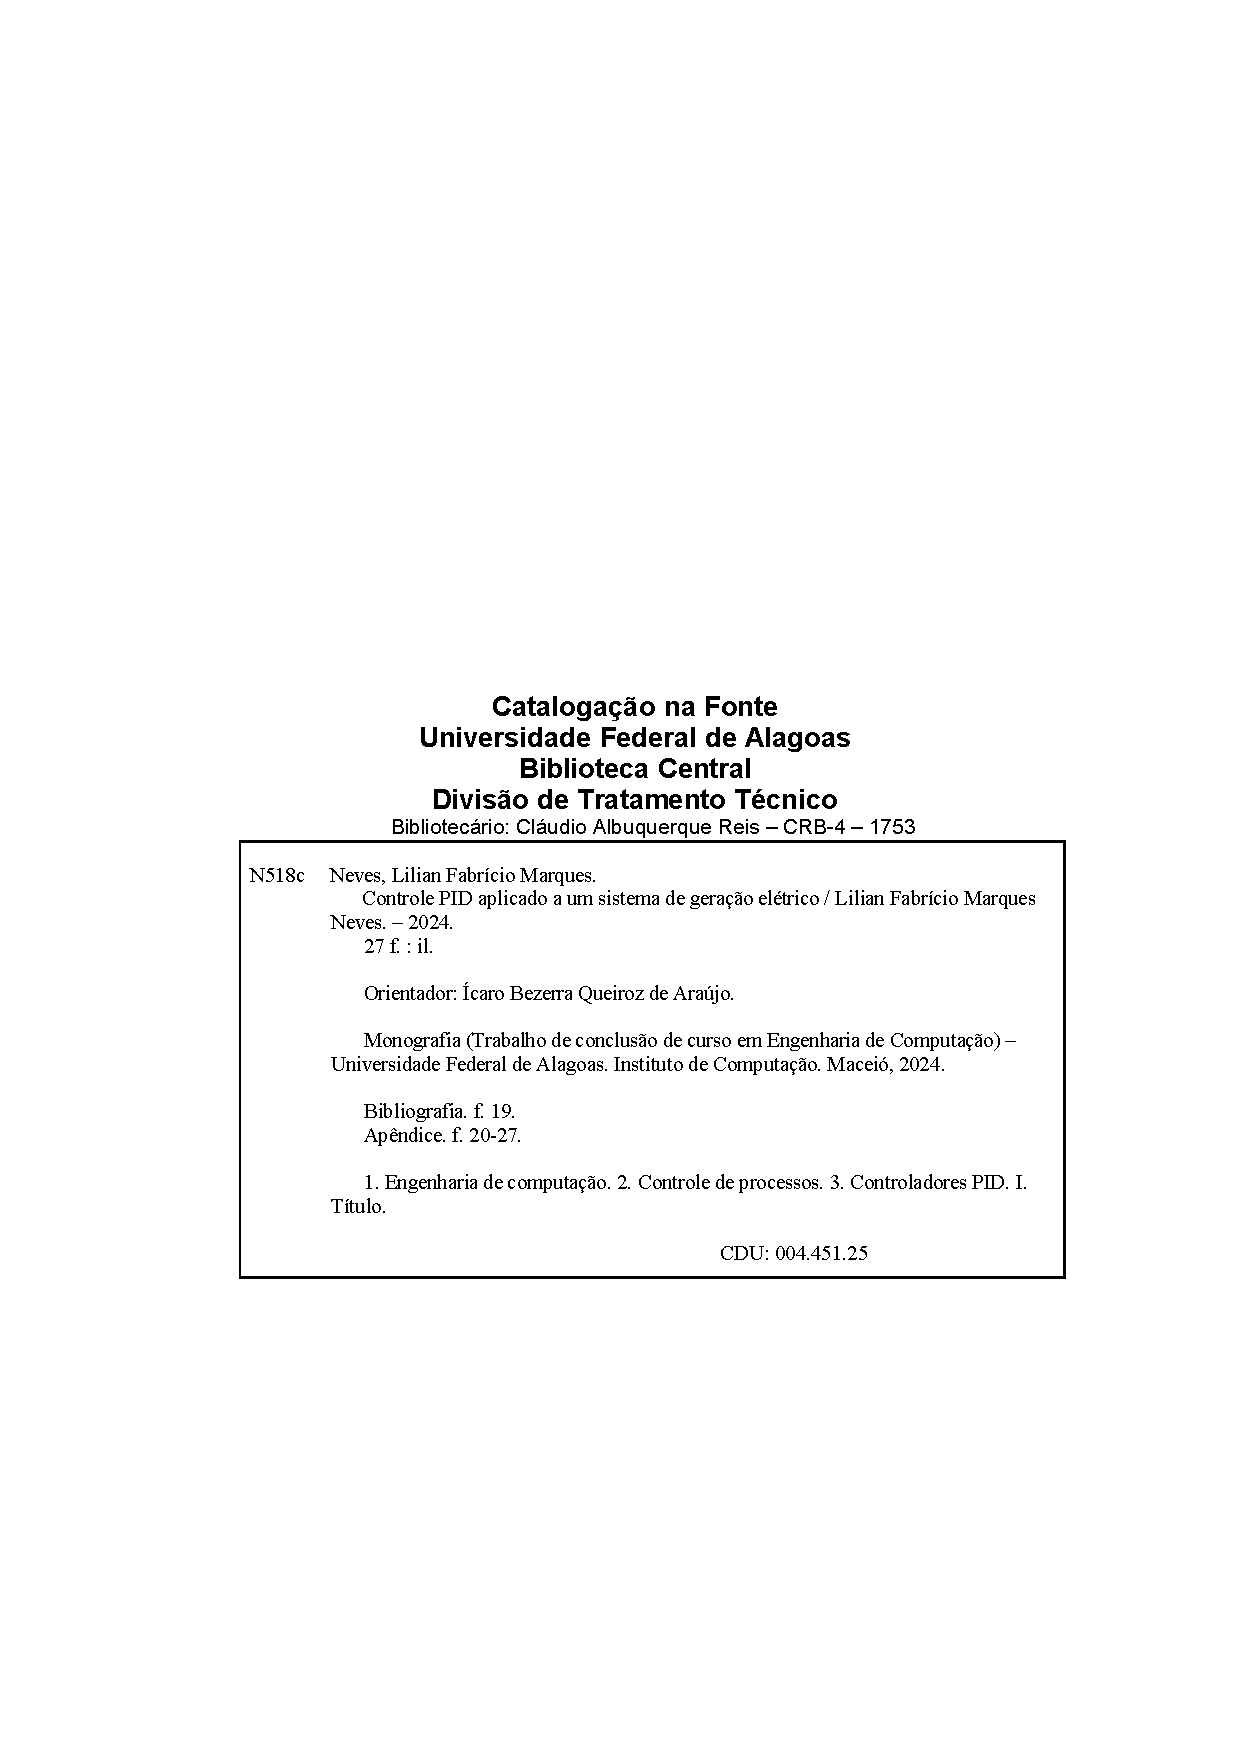
\includepdf{Cap00/Ficha Catalografica.pdf}
%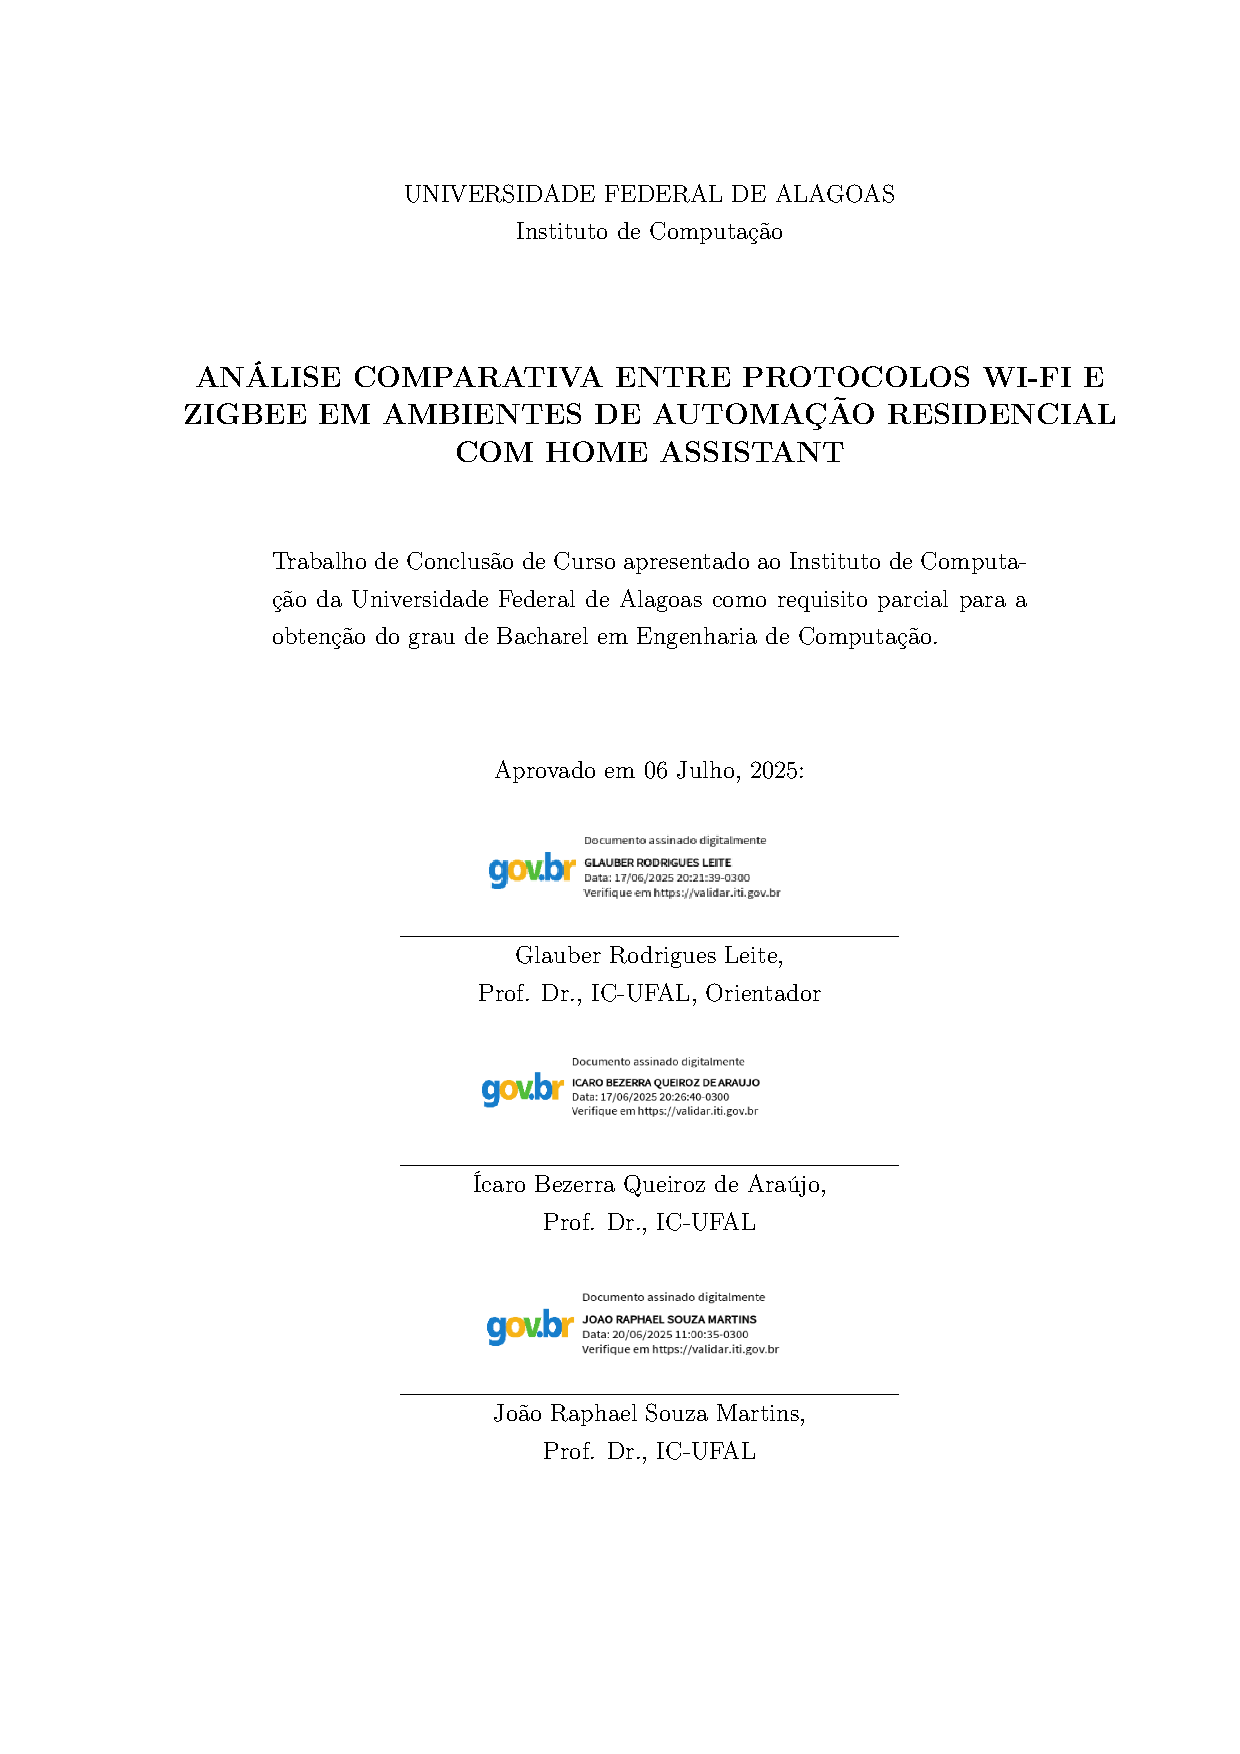
\includepdf{Cap00/TCC_FORMULARIO.pdf}
\folhaDeAprovacao

% % % % % % % % % % % % % % % % % % % % % % % % % % %
% Opcionais % % % % % % % % % % % % % % % % % % % % %
% % % % % % % % % % % % % % % % % % % % % % % % % % %
\dedicatoria %opcional
% \agradecimentos %opcional
%\epigrafe %opcional



% % % % % % % % % % % % % % % % % % % % % % % % % % %
% Obrigatórios  % % % % % % % % % % % % % % % % % % % 
% % % % % % % % % % % % % % % % % % % % % % % % % % %
\resumo
\abstract
% % % % % % % % % % % % % % % % % % % % % % % % % % %
% % % % % % % % % % % % % % % % % % % % % % % % % % %
\listoffigures
\cleardoublepage
% % % % % % % % % % % % % % % % %
%\listoftables
\cleardoublepage
%\simbolos
\cleardoublepage
\abreviaturas
\cleardoublepage
% % % % % % % % % % % % % % % % % % % % % % % % % % %
% % % % % % % % % % % % % % % % % % % % % % % % % % %
%\renewcommand{\contentsname}{Summary}
\tableofcontents
\cleardoublepage
% % % % % % % % % % % % % % % % % % % % % % % % % % %
% % % % % % % % % % % % % % % % % % % % % % % % % % %
\pagenumbering{arabic}

\pagestyle{myheadings}
\renewcommand{\chaptermark}[1]{\markboth{#1}{}}
\renewcommand{\sectionmark}[1]{\markright{#1}}
%% Remover depois
\chapter{Dicas}

Dicas de uso de citação, equações, figuras e tabelas

\subsection{Citação}
Lembre de adicionar as referências no arquivo .bib

Citação direta... Segundo \cite{accardi2012}.

Citação indireta... \citep{accardi2012}

\subsection{Equações}

Dê uma olhada no arquivo macros.tex e adicione o que tiver interesse. Lembre sempre de referenciar equações numeradas. (...) como pode ser visto na Equação \ref{eq:teste}.

\begin{equation}
    \stateStart = \begin{bmatrix}
        \cos{\phi} & \sin{\phi} & 0
    \end{bmatrix}^\top \in \set{\Omega} \subset \R^3
    \label{eq:teste}
\end{equation}

Também é possível montar uma equação multilinha, como pode ser visto em \ref{eq:problem_mpc}.
\begin{equation}
    \begin{split}
        \text{minimizar} & \quad \sum_{k = 0}^{k = N} (\stateVec(k) - \refVec(k))^\top \matr{Q}(k) (\stateVec(k) - \refVec(k)) + \sum_{k = 0}^{k = N - 1} \inputVec(k)^\top \matr{R}(k) \inputVec(k), \\
        \text{sujeita a} & \quad \stateVec(k+1) = \matr{F} \stateVec(k) + \matr{G} \inputVec(k), \\
        & \quad \stateVec_{\min} \leq \stateVec(k)\leq \stateVec_{\max}, \\
        & \quad \inputVec_{\min} \leq \inputVec(k)\leq \inputVec_{\max}, \\
        & \quad \stateVec(0) = \stateVec_0.
    \end{split}
    \label{eq:problem_mpc}
\end{equation}

\subsection{Figuras}

Lembre de sempre referenciar figuras. (...) Como pode ser visto na Figura \ref{fig:imagemEstande}.

\begin{figure}[H]
    \centering
    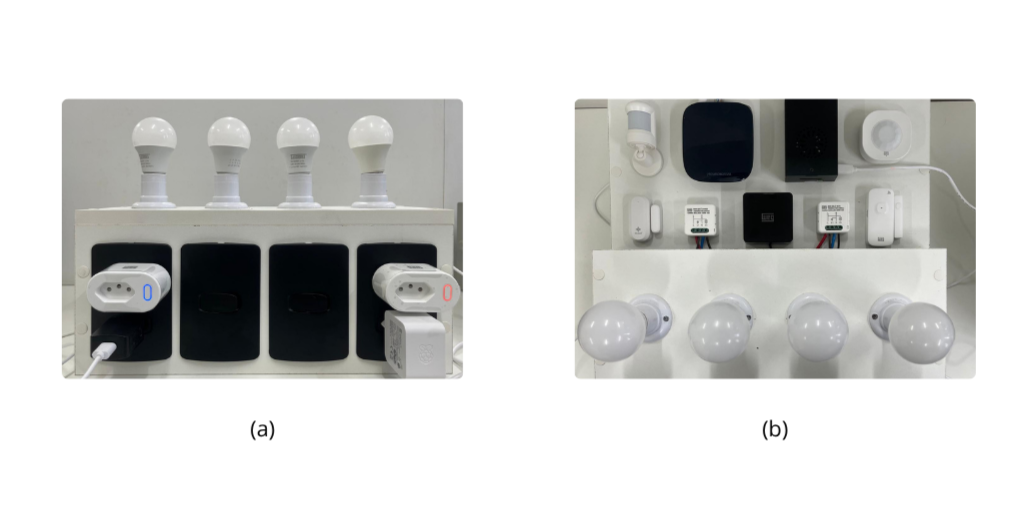
\includegraphics[width=\linewidth]{Cap03/img/vistaEstande.png}
    \caption{Fotos do Estande desenvolvido para aplicação: (a)Vista Frontal - Disposição de tomadas, tomadas inteligentes e interruptores; (b) Vista Superior - Disposição das lâmpadas, sensores, atuadores e controladores.}
    \label{fig:imagemEstande}
\end{figure}

\subsection{Tabela}

Lembre de sempre referenciar tabelas. (...) Como pode ser visto na Tabel \ref{tab:devices}.

\newcolumntype{P}[1]{>{\centering\arraybackslash}p{#1}}
\begin{table}[h]
    \centering
    \renewcommand{\arraystretch}{1.5} % aumenta altura das linhas
    \begin{tabular}{P{4cm}P{2cm}P{2.8cm}P{5cm}}
        \hline
        \textbf{Dispositivo} & \textbf{Protocolo} & \textbf{Marca} & \textbf{Função} \\
        \hline
        Roteador Wi-Fi & Wi-Fi & Tp-Link & Roteamento da rede e conexão com a internet \\
        Hub Zigbee & Zigbee & Nova Digital & Coordenador da rede Zigbee\\
        Sensor de Porta & Wi-Fi & WEG & Detecção de abertura/fechamento \\
        Sensor de Movimento & Wi-Fi & WEG & Detecção de movimento \\
        Sensor de Porta & Zigbee & Ekasa & Detecção de abertura/fechamento \\
        Sensor de Movimento & Zigbee & Nova Digital & Detecção de movimento \\
        Relé inteligente & Wi-Fi & WEG & Controle de carga via Wi-Fi \\
        Tomada inteligente & Wi-Fi & WEG & Acionamento remoto de equipamentos\\
        Relé inteligente & Zigbee & WEG & Controle de carga via Zigbee \\
        Tomada inteligente & Zigbee & WEG & Acionamento remoto de equipamentos\\
        Central de Automação & - & Raspberry Pi 5 & Execução do Home Assistant \\
        \hline
    \end{tabular}
    \caption{Lista de dispositivos do estande}
    \label{tab:devices}
\end{table}

% % % % % % % % % % % % % % % % % % % % % % % % % % %
% Incluir capítulos aqui  % % % % % % % % % % % % % %
% % % % % % % % % % % % % % % % % % % % % % % % % % %
\chapter{Introdução}\label{cap:introducao}

\lipsum[1-4]

\section{Objetivos}

Objetivo geral

\subsection{Objetivos Específicos}
\begin{itemize}
\item Objetivo Específico 1

\item Objetivo Específico 2

\item Objetivo Específico 3

\end{itemize}

\section{Organização do trabalho}

\lipsum[1]
\cleardoublepage
% % % % % % % % % % % % % % % % % % % % % % % % % % %
\chapter{Fundamentação Teórica}\label{cap:fundamentacao}

\lipsum[1-6]
\cleardoublepage
% % % % % % % % % % % % % % % % % % % % % % % % % % %
\chapter{Metodologia}\label{cap:metodologia}

\lipsum[7-12]
\cleardoublepage
% % % % % % % % % % % % % % % % % % % % % % % % % % %
\chapter{Resultados e Discussões}\label{cap:resultados}

\lipsum[13-18]
\cleardoublepage
% % % % % % % % % % % % % % % % % % % % % % % % % % %
%\input{Cap05/Capitulo5}
%\cleardoublepage
% % % % % % % % % % % % % % % % % % % % % % % % % % %
%\input{Cap06/Capitulo6}
%\cleardoublepage
%%% % % % % % % % % % % % % % % % % % % % % % % % % % %

\chapter{Conclusão}\label{sec:conclusao}

\lipsum[1-3]
\cleardoublepage
%%% % % % % % % % % % % % % % % % % % % % % % % % % % %
%%% % % % % % % % % % % % % % % % % % % % % % % % % % %
\markright{Bibliography}
%\renewcommand\bibname{Bibliography}

% % % % % % % % % % % % % % % % % % % % % % % % % % %
% Definir estilo bibliográfico  % % % % % % % % % % %
% % % % % % % % % % % % % % % % % % % % % % % % % % %

%\bibliographystyle{alpha}
\bibliographystyle{apalike}
%\bibliographystyle{ieeetr}
%%
{
	\addcontentsline{toc}{chapter}{Bibliografia}
	\bibliography{Ref/SampleReferences}
}
\cleardoublepage
%%% % % % % % % % % % % % % % % % % % % % % % % % % % %
%%% % % % % % % % % % % % % % % % % % % % % % % % % % %

\appendix
\chapter{Script de Coleta de Dados MQTT em Python}

\begin{lstlisting}[language=Python, basicstyle=\ttfamily\small, breaklines=true]
import paho.mqtt.client as mqtt
import csv, os, sys

CENARIOS_ATIVOS = [
    ["MZ", "RZ", "ON", "OFF"],
    ["MZ", "RZ", "OFF", "ON"],
]
BUFFER, COUNT = [], 0

def save(index, t1, t2):
    d1, d2, s1, s2 = SCENARIOS[index]
    path = os.path.join("BASE_DIR", f"{d1}_{d2}", f"{s1}_{s2}.csv")
    with open(path, "a", newline="") as f:
        csv.writer(f).writerow([t1,t2])

def handle_messages(BUFFER):
    timers = [BUFFER.split()[1] for l in BUFFER]
    save(0,timers[0], timers[1])
    save(1,timers[2],timers[3])

def on_connect(client, userdata, flags, rc):
    client.subscribe("TOPIC_DEFINE")

def on_message(client, userdata, msg):
    global BUFFER, COUNT
    BUFFER.append(msg.payload.decode())
    if len(BUFFER) == 4:
        handle_messages(BUFFER)
        BUFFER, COUNT = [],COUNT + 1
        if COUNT == 20:
            print("Coleta completa.")
            client.loop_stop()
            sys.exit(0)

def main():
    global client
    client = mqtt.Client()
    client.username_pw_set("MQTT_USERNAME", "MQTT_PASSWORD")
    client.on_connect = on_connect
    client.on_message = on_message
    client.connect("MQTT_BROKER", "MQTT_PORT", 60)
    print("MQTT Ativo...")
    client.loop_forever()

if __name__ == "__main__":
    main()
\end{lstlisting}

\cleardoublepage

\end{document}
